%%%%%%%%%%%%%%%%%%%%%%%%%%%%%%%%%%%%%%%%%%%%%%%%%%%%%%%%%%%%%%%%%%%%%%%%%%%
%
% Fuzzy time domain
%
%%%%%%%%%%%%%%%%%%%%%%%%%%%%%%%%%%%%%%%%%%%%%%%%%%%%%%%%%%%%%%%%%%%%%%%%%%%
%INTRO
As explained in the introduction, humans handle temporal information using temporal notions like time intervals or time points \cite{Dyreson1994}. While the used temporal notions may contain imperfections~\cite{Dev98},~\cite{Dubois:jucs_9_9:fuzziness_and_uncertainty_in},~\cite{nagypal2003},~\cite{Dubois89}, humans often gracefully deal with these, as their inherent interpretation capability accounts for a lot of them. This phenomenon has been studied a.o. in the field of artificial intelligence~\cite{Tre97},~\cite{5151} and language understanding~\cite{DeCaluwe:1997:FTI:285506.285516},~\cite{nagypal2003},~\cite{Dev98}. An information system, however, cannot appeal to a similar interpretation functionality. Thus, many proposals have been concerned with the combination of time and imperfections in the context of information systems~\cite{nagypal2003}. In this section, some main concepts and issues concerning this combination are presented.


\subsection{\label{subsec:representation}Representation}

As mentioned before, humans deals with time with vagueness. Even for some specific events or facts, the temporal specification becomes imprecise. Therefore, as a result of the imprecise managment of the time that humans do, a time point is specified or managed by means of a time interval which boundaries may not be precissely known.

\begin{example}
Consider a speaker and a hearer. The speaker wants to make an appointment with the hearer. Consider now that the speaker says:\\
\begin{center}
\emph{`We will meet each other tomorow around 10'}\\
\end{center}
The hearer usually agree that the appointment will be in the time interval 9.55 to 10.05.
\end{example}

The study of the semantics of `around' in temporal~\cite{Dev98} indications has shown that also the size of the temporal interval associated with the imprecise specification of the time depends on the distance with respect to the current time. E.g. Consider now that the speaker is talking about something that happened \emph{`during last week'} then the hearer would consider a time interval of more or less 10 days. 


Some proposals ~\cite{knight1993},~\cite{Cru97},~\cite{nagypal2003},~\cite{Chountas2000} conclude that the best representation for incomplete temporal knowledge are therefore time intervals even if they refer to a fact that happen in a time point. This means that, as Allen proprosed in \cite{Allen83} the primitive units (the chronons) in the temporal system are intervals.

In order to manage uncertain temporal information properly, several theoretical frameworks have been proposed:

\begin{description}
\item[\emph{Probability theory}]
The probability theory~\cite{Dey1996},~\cite{Lakshmanan1997},~\cite{Haddawy1996} is employed when a probability is associated to the time interval. It is very usual in logistics information systems. e.g. \emph{`The package will arrive at its destination on monday morning with a probability of 0.8'}.



\item[\emph{Possibility theory}]
The possibility theory~\cite{Zadeh65} associates a possibility degree to the temporal fact or event. This theoretical framework is widely used to model uncertainty and vaguenes in time~\cite{Dubois:jucs_9_9:fuzziness_and_uncertainty_in},\cite{Dubois89},\cite{devos94},\cite{nagypal2003}. Several works~\cite{schockaert08},~\cite{ohlbach2004} presents a fuzzy version of the temporal relations given by Allen~\cite{Allen83}. The aim of these works is to obtain a flexible way to compare uncertain, ill-known temporal intervals by means of the temporal relationships.


\item[\emph{Rough sets}]
Rough set theory~\cite{Pawlak1995} has been used to represent uncertainty in time intervals. The two dimensional representation of time intervals and the temporal relationships between them has been studied in~\cite{Qia09}.
\end{description}


%\subsection{\label{subsec:classification}Classification of imperfect temporal information}


\subsection{Types of Imperfections in Temporal Modelling}
Generally, in temporal modelling, a distinction is made between the following types of imperfections~\cite{nagypal2003}.


\begin{itemize}
	\item \emph{Uncertainty}: Temporal information or data may contain uncertainty. This means that the exact temporal value is (partially) unknown, however, generally some knowledge is present anyhow, possibly describing the value~\cite{Dubois:jucs_9_9:fuzziness_and_uncertainty_in},~\cite{nagypal2003},~\cite{Dubois89},~\cite{343607}. E.g., the temporal notion described in a sentence like `The Belfry of Bruges was finished on a day somewhere between 01/01/1201 A.D. and 31/12/1300 A.D.' contains uncertainty: it is known that the belfry of Bruges was finished on a single day and that this day lays somewhere between 01/01/1201 A.D. and 31/12/1300 A.D., but it is not known exactly which day it is.
	\item \emph{Vagueness}: Temporal information or data might contain inherent vagueness, as a precise instant or time interval may be intended, but the description of it is certainly vague~\cite{schockaert08},~\cite{nagypal2003},~\cite{Dev98}. E.g., the temporal notion described in a sentence like `It happened during summer.' contains vagueness, as even the boundaries of the mentioned temporal notion are not clearly expressed.
	\item \emph{Subjectivity or ambiguity}: Temporal notions might be subject to subjectivity or ambiguity. In certain cases, the temporal notion concerns a historical period like `late romanticism' or `the early middle ages' and thus contains subjectivity~\cite{nagypal2003}. In other cases, the interpretation of the temporal notion depends on extra factors. E.g., consider a person saying to another person `Let's meet each other at six.' The person hearing these words doesn't now if 6 a.m. or 6 p.m. is intended, though the person saying the words does.
\end{itemize}

As to the sources of the imperfections in temporal information, most proposals consider no specific source~\cite{5151},~\cite{schockaert08},~\cite{nagypal2003},~\cite{Dubois89},~\cite{343607},~\cite{ohlbach2004},~\cite{Virant199639}. Some proposals, however, deal with the imperfections specifically resulting from aspects of language~\cite{Dev98} and other proposals consider transitions between different granularities to be the source of imperfection in temporal information~\cite{Lin97}. Therefore, some proposals consider granularity as the base of the temporal model~\cite{Cru97}.



Temporal information is usually related to facts or events~\cite{Chountas2000}. Therefore, the following types of temporal information may be found:

\begin{description}
\item[\emph{Definite temporal information}]
It is found when all times associated with the fact are absolute times. The temporal information is precisely known.

\item[\emph{Indefinite temporal information}]~\cite{Dey1996}
The time associated with the fact has not been fully defined. Consider an event that in fact occur but it is not known exactly when.

\item[\emph{Infinite temporal uncertain information}]~\cite{Kabanza1990}
An infinite number of times are associated with a fact. This is usually found in recurrent events like meetings. (e.g. \emph{The meetings are every Wednesday at noon.}). Some systems (usually with different information providers) may dispute the occurence of a fact and / or the duration of a fact. 
\end{description}


\subsection{Imperfections in Temporal Relationships}
As the existence of temporal relationships allows to compare temporal notions, many approaches have been concerned with finding similar temporal relationships, able to support imperfections in the temporal information which is described by temporal notions or even by the temporal relationships themselves~\cite{ohlbach2004},~\cite{nagypal2003},~\cite{schockaert08},~\cite{Dubois:jucs_9_9:fuzziness_and_uncertainty_in}. These approaches are often based on Allen's operators~\cite{Allen83}. Example \ref{ex:fuzzy-allen-relation} is a case of use for one of the Allen's relations.


\begin{example}
\label{ex:fuzzy-allen-relation}
Consider an event which is bounded at $[A,B]$ both the starting and ending points respectively (see (1) in figure \ref{fig:fuzzy-allen-relationship} ). The classical Allen's after relation returns an interval from $]B,\infty[$ as shown in (2) in figure \ref{fig:fuzzy-allen-relationship}. A fuzzified version of the Allen's operators is illustrated in (3), figure \ref{fig:fuzzy-allen-relationship}. The comparison between two time intervals results in a possibility degree in the unit interval. The shape for the membership function is shown in (3), figure \ref{fig:fuzzy-allen-relationship}. Note that all the points strictly after the point $B$ results in a possibility degree of 1 whereas there is an area near the point $B$ in which the possibility degree runs smoothly between 0 and 1. 

Consider now the interval given by $[C,D]$, illustrated in (4), figure \ref{fig:fuzzy-allen-relationship}. The user wants to know if $[C,D]$ is after $[A,B]$. The crisp version of the \emph{`after'} operator would return \emph{`no'} as an answer. The fuzzy version for the same operator would return \emph{`yes, with a possibility of 0.5'}.


\begin{figure}
\centering
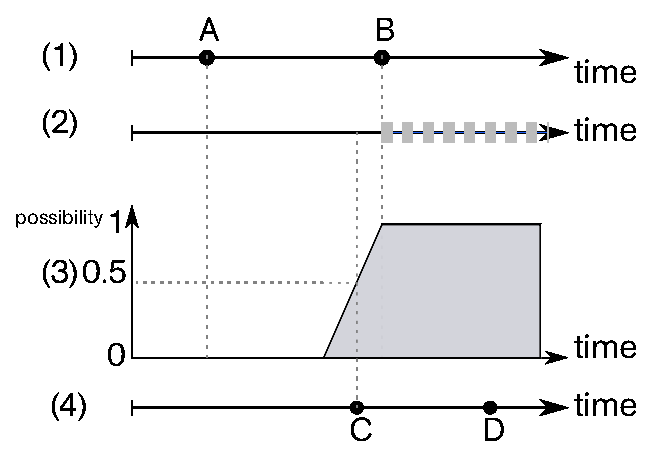
\includegraphics[scale=0.5]{graphs/fuzzyAllen.eps}
\caption{Example for the Allen's relation, \emph{`after'}. (1) The event bounded within the time points $A$ and $B$. (2) The crisp version for the \emph{`after'} operator. (3) A fuzzy version for the after operator. (4) Another event bounded within the time points $[C,D]$.}
\label{fig:fuzzy-allen-relationship}
\end{figure}
\end{example}




%%%%%%%%%%%%%%%%%%%%%%%%%%%%%%%%%%%%%%%%%%%%%%%%%%%%%%%%%%%%%%%%%%%%%%%%%%%
%
% End fuzzy time domain
%
%%%%%%%%%%%%%%%%%%%%%%%%%%%%%%%%%%%%%%%%%%%%%%%%%%%%%%%%%%%%%%%%%%%%%%%%%%%%%